\documentclass[a4paper,12pt]{article}

\usepackage{graphicx}
\usepackage{float}
\usepackage[utf8]{inputenc}
\usepackage{booktabs}
\usepackage{siunitx}
\usepackage{geometry}
\geometry{margin=2.5cm}


\sisetup{
    table-format=2.2,
    round-mode=places,
    round-precision=2
}



\title{Report 3 - Logistic Regression}
\author{Le Nghiem Thanh Thuy}
\date{May 2026}

\begin{document}

\maketitle

\section{Algorithm}
In this report I use Logistic Regression to classify 2 class on a small dataset (50 points, 2 features X1 and X2). The model is:
\[
\hat{y} = \sigma(w_1 x_1 + w_2 x_2 + w_0), \quad \sigma(z) = \frac{1}{1 + e^{-z}}
\]

Loss function is Cross Entropy:
\[
L = -\frac{1}{n}\sum_{i=1}^{n} \big[ y_i \log(\hat{y}_i) + (1 - y_i)\log(1 - \hat{y}_i) \big]
\]

I use gradient descent to update the weights $w_1, w_2, w_0$ each epoch. The training stop when the loss change is smaller than the threshold.

Initial value: $w_1 = 1.0$, $w_2 = 1.0$, $w_0 = 0.0$. Learning rate = 0.001, threshold = 0.000001, max epochs = 100000.

Model converge at epoch 65931 with final loss $\approx 0.1158$ and weights $w_1 = 0.6767$, $w_0 = -4.8414$.



\section{Result}

After training, I draw the decision boundary and also plot the loss curve to check the convergence.

The test point $x_1 = 6, x_2 = 4$ give the prediction $\hat{y} \approx 0.6683$, so it belong to class 1.


\begin{figure}[H]
    \centering
    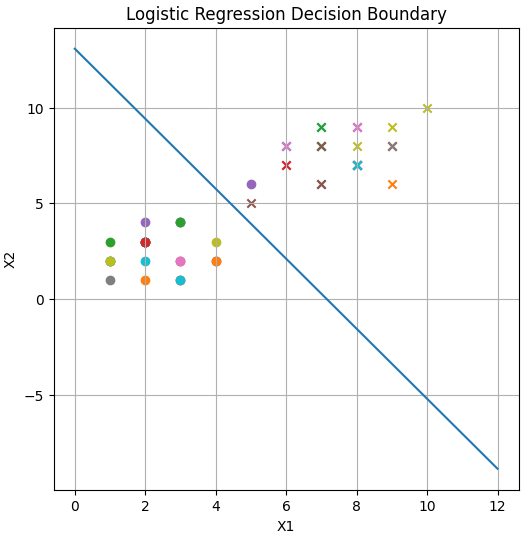
\includegraphics[width=0.6\textwidth]{LogR_Result.png}
    \caption{Decision boundary of the model}
    \label{fig:logr_result}
\end{figure}


\begin{figure}[H]
    \centering
    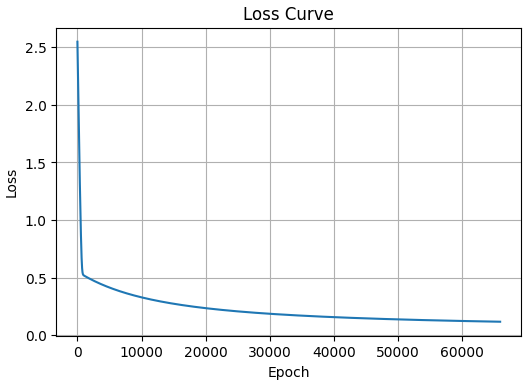
\includegraphics[width=0.6\textwidth]{LogR_Loss.png}
    \caption{Loss of model over epochs}
    \label{fig:logr_loss}
\end{figure}


\end{document}
